\documentclass{article}
\usepackage{amsmath}
\usepackage{amsfonts}
\usepackage{amssymb}
\usepackage{enumitem}
\usepackage{tikz}
\usepackage{mathtools}

\title{MATH 222 - Assignment 2}
\date{February 2017}
\author{Daniel Frankcom}

\begin{document}
	\pagenumbering{gobble}
	\maketitle
	\setlength{\parindent}{0pt}
	\newcommand{\forceindent}{\leavevmode{\parindent=72pt\indent}}
	\newpage
	\pagenumbering{arabic}
	
	\begin{enumerate}
		\item Since the partition that a given vertex belongs to is determined by the number of 1s in the sequence, the beginning vertex (00...0) will always be in $V_2$. Dissimilarly however, the ending vertex (11...1) will fluctuate depending on the value of n, as it will contain an even number of 1s if n is even, and will contain an odd number of 1s if n is odd.
		\newline For this reason, when n is even the starting and ending node will be in the same partition.
		\newline Since there are an even number of vertices in each partition, it is not possible to start on 00...0 and zig-zag between the partitions without ending up in the opposite partition to our start vertex and our desired end vertex.
		\newline $\therefore$ there is only a Hamiltonian path in $Q_n$ when n is odd.
		
		\item If there exists a $u-w$ path of $G$ not containing $v$, then $G-v$ would still be 1 connected component, meaning that $v$ is not a cut-vertex. Similarly, if there is not a $u-w$ path containing $v$, then $v$ will not affect the connection between these vertices, and $v$ will not be a cut-vertex.
		
		\item
		\begin{enumerate}
			\item $K_5$ is a complete graph, meaning that any graph $G-e$ will be isomorphic to every other possible version of $K_5$ with one edge removed. Since all such versions of $K_5-e$ are isomorphic, we only need to show that one such version is planar:
			\newline\newline
			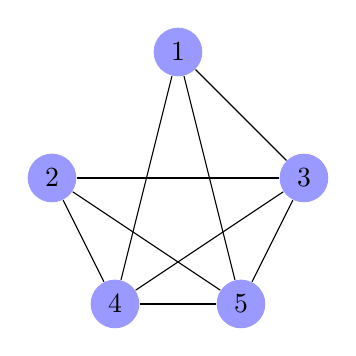
\begin{tikzpicture}
			[scale=.8,auto=left,every node/.style={circle,fill=blue!40}]
			\node (n1) at (2,4)  {1};
			\node (n2) at (0,2)  {2};
			\node (n3) at (4,2)  {3};
			\node (n4) at (1,0)  {4};
			\node (n5) at (3,0)  {5};
			
			\foreach \from/\to in {n2/n4,n4/n5,n5/n3,n1/n3,n1/n4,n1/n5,n2/n5,n2/n3,n3/n4}
			\draw (\from) -- (\to);
			\end{tikzpicture}
			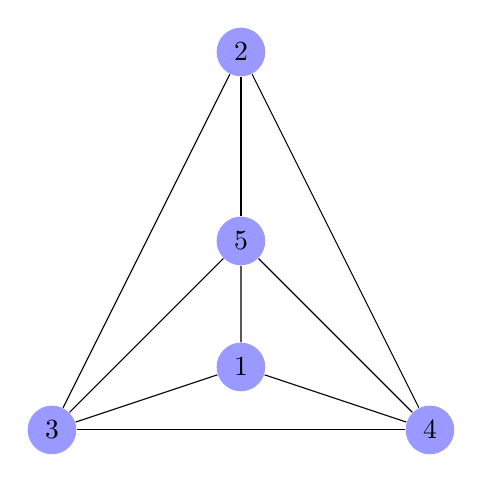
\begin{tikzpicture}
			[scale=.8,auto=left,every node/.style={circle,fill=blue!40}]
			\node (n1) at (3,1)  {1};
			\node (n2) at (3,6)  {2};
			\node (n3) at (0,0)  {3};
			\node (n4) at (6,0)  {4};
			\node (n5) at (3,3)  {5};
			
			\foreach \from/\to in {n2/n4,n4/n5,n5/n3,n1/n3,n1/n4,n1/n5,n2/n5,n2/n3,n3/n4}
			\draw (\from) -- (\to);
			\end{tikzpicture}
			\newline
			\item Using the theorem $|E|\leq 3|V|-6$, both conditions below must hold.
			\begin{itemize}
				\item The following is true in $G$:
				\newline $|E|\leq3(11)-6$
				\newline $|E|\leq33-6$
				\newline $|E|\leq27$
				\newpage
				\item Then the following is true in $\bar{G}$:
				\newline $\frac{11(11-1)}{2}-27\leq3(11)-6$
				\newline $\frac{110}{2}-27\leq33-6$
				\newline $55-27\leq27$
				\newline $28\leq27$
				\newline This statement is untrue
			\end{itemize}
			$\therefore |V|$ must be less than 11
		\end{enumerate}
	
		\item If $G$ has no cycles, then it is possible to traverse the graph, alternating colours at each adjacent vertex in order to obtain a 2-colouring. If $G$ has exactly one cycle, then it may still be possible to create a 2-colouring, however if $G$ contains an odd cycle, then we will require 3 colours, as there will be a single vertex that is adjacent to both of the previously used colours.
		
		\item If $\chi\le4$, then $G$ is planar.
		\newline This statement is not true, as $K_{3,3}$ is non-planar and since it is bipartite, it has a chromatic number of 2, which is less than 4.
		
		\item Since $T$ contains no cycles (definition of a tree), for any given node, all vertices will surely end in a leaf. $T$ may have more than $k$ leaves, as a branch may split into more than 1 leaf if one of the proceeding vertices is greater than degree 1.
	
		\item ${{2n}\choose{2}}$ is equivalent to counting the number of ways to choose 2 items from a set that is twice the size of a set n.
		\newline On the other side of the equation:
		\newline ${{n}\choose{2}}$ is equivalent to choosing 2 elements from a set of size n, and we multiply it by 2 because we have 2 sets of size n.
		\newline We then add $n^2$, since this is equivalent to choosing 1 element from each sets of size n.
		\newline
		\newline By example:
		\newline The number of choices of 2 cards from 2 decks is the same as 2 times the number of choices from 1 deck, plus the number of choices of 1 card from each deck.
		
		\item
		\begin{enumerate}
			\item This expression is equivalent to $\sum\limits_{k=0}^n{{n}\choose{k}}2^k$
			\newline The above resembles the formula $\sum\limits_{k=0}^n{{n}\choose{k}}x^ky^{n-k}$, with $y=1$ and $x=2$
			\newline $\therefore$ the expression can be simplified to $(2+1)^n=3^n$
			
			\newpage
			\item Suppose there is a set of $n$ people, some of which will be rejected, some of which will be accepted into a university, and some of which will be put straight into the honors class. We can choose any number of people and put them into any one of the 3 groups, however they may not be in more than 1 group.
			\newline We can select ${n\choose0}+\cdots+{n\choose n}$ people to get into the university, however we must also decide how many people we allow into the honors class, hence the $2^k$ in front of every choice.
			\newline Alternatively, there are 3 possible groups for people to be split into, so we have 3 options per $n$ people, hence there are $3^n$ possible ways to arrange them into the groups.
		\end{enumerate}
	
	\end{enumerate}
\end{document}